\documentclass[11pt]{article}

% --- Encoding & fonts (matches series style) ---
\usepackage[utf8]{inputenc}
\usepackage[T1]{fontenc}
\usepackage{lmodern}
\usepackage[protrusion=true,expansion=false]{microtype}
\setlength{\emergencystretch}{3em}

% --- Page geometry ---
\usepackage[margin=1in, top=1.1in, bottom=1.1in]{geometry}

% --- Packages ---
\usepackage{amsmath,amssymb,amsthm}
\usepackage{booktabs}
\usepackage{graphicx}
\usepackage[colorlinks=true,
            linkcolor=blue!70!black,
            citecolor=blue!70!black,
            urlcolor=blue!70!black]{hyperref}
\usepackage{xcolor}
\usepackage{enumitem}
\usepackage[numbers,sort&compress]{natbib}
\usepackage{caption}
\captionsetup{font=small,labelfont=bf}
\usepackage{tikz}
\usetikzlibrary{shapes.geometric,arrows.meta,positioning,fit,backgrounds}
\usepackage{multirow}
\usepackage{array}

% --- Section formatting ---
\usepackage{titlesec}
\titleformat{\section}{\large\bfseries}{\thesection}{1em}{}
\titleformat{\subsection}{\normalsize\bfseries}{\thesubsection}{1em}{}

% --- Paragraph spacing ---
\setlength{\parskip}{0.5em}
\setlength{\parindent}{0pt}

% --- Theorem environments ---
\newtheorem{theorem}{Theorem}[section]
\newtheorem{lemma}[theorem]{Lemma}
\newtheorem{corollary}[theorem]{Corollary}
\newtheorem{proposition}[theorem]{Proposition}
\newtheorem{definition}{Definition}[section]
\newtheorem{remark}{Remark}[section]

% --- Notation ---
\newcommand{\Azero}{\mathcal{A}_0}
\newcommand{\Dhat}{\widehat{D}}
\newcommand{\Sp}{S_p}
\newcommand{\Sr}{S_r}
\newcommand{\calF}{\mathcal{F}}
\newcommand{\CW}{\mathrm{CW}}
\newcommand{\IER}{\mathrm{IER}}
\newcommand{\SHR}{\mathrm{SHR}}
\newcommand{\OCR}{\mathrm{OCR}}
\newcommand{\ADMIT}{\texttt{ADMIT}}
\newcommand{\ESCALATE}{\texttt{ESCALATE}}
\newcommand{\DENY}{\texttt{DENY}}
\newcommand{\EXECUTE}{\texttt{EXECUTE}}
\newcommand{\HALT}{\texttt{HALT}}
\newcommand{\RESUME}{\texttt{RESUME}}
\newcommand{\RS}{\mathrm{RS}}

% --- Title ---
\title{\textbf{Runtime Governance for LLM-Based Agent Systems}\\[4pt]
       \large Applying the Agent Governance Stack to Real Agentic Workflows}

\author{Marcelo Fernandez\\
        \small TraslaIA\\
        \small \texttt{info@traslaia.com}}
\date{}

% =============================================================================
\begin{document}
\maketitle

% --- Abstract -----------------------------------------------------------------
\begin{abstract}
Autonomous agent systems built on large language models require runtime
governance mechanisms that are formal, stateful, and composable -- not merely
heuristic.
Existing approaches (prompt guards, OPA/XACML policy engines, audit layers)
share a common structural weakness: they evaluate actions locally and cannot
detect behavioral drift that is invisible within any individual rule evaluation.
This paper presents the first empirical validation of the complete Agent
Governance Stack -- a seven-paper formal series (P0--P6) covering atomic
decision boundaries, stateful admission control (ACP), invariant measurement
(IML), governance structure, reconstructive authority (RAM), and its
operationalization -- applied to real \textbf{LangGraph} agent workflows.
We implement all four components of the stack (ACP gate, IML monitor, RAM
gate, Recovery Loop) as a Python library instrumented into a three-node
LangGraph StateGraph, and run four targeted experiments.
Our results confirm the theoretical predictions with zero deviation:
(1)~IML detects compliant drift invisible to ACP in all six seeds, with
detection step $T^*\in[259,403]$;
(2)~the RAM gate achieves $\IER=0.000$ across all state-coverage levels
$(0.10$--$1.00)$, versus baseline $\IER\in[0.032,\,0.185]$;
(3)~the ACP coordination window replicates $\CW_{\mathrm{appr}}=2N$ with
zero deviation for $N\in\{2,4,8,16\}$ agents, confirming Paper~1
Experiment~13 in Python/LangGraph;
(4)~the full integrated stack converges with $\Dhat$ bounded in $[0.27,0.34]$
over 2000 steps, liveness holds, and no deadlock occurs.
We also report three empirical findings that refine the theoretical
framework: a type mismatch between ACP's baseline-RS model and
tool-intrinsic risk scores, a recoverable-vs-irresolvable HALT
classification for the conditional liveness theorem, and an
EMA-parameter dependency in the convergence bound.
Code and data are available at:
\url{https://github.com/chelof100/agent-governance-applied}.
This is Paper~7 of the 8-paper Agent Governance Series.
\end{abstract}

\tableofcontents
\newpage

% =============================================================================
\section{Introduction}
\label{sec:intro}

Autonomous agent systems built on large language models (LLMs) are increasingly
deployed in production settings where they execute consequential actions:
modifying data, invoking APIs, delegating subtasks to other agents, and
coordinating across shared resources~\cite{yao2023react,weng2023agent}.
The governance question -- \emph{who controls what the agent may do, and how is
that control enforced at runtime?} -- has grown urgent as these systems move
from research prototypes to production pipelines.

Current approaches share a common design pattern: they evaluate agent actions
locally, at the point of execution, against a fixed rule set.
\emph{Prompt guards} check model outputs for policy violations before
passing them downstream.
\emph{OPA/XACML policy engines}~\cite{openpolicyagent2023,anderson2004extensible}
evaluate capability tokens against attribute-based access rules.
\emph{Constitutional AI}~\cite{bai2022constitutional} uses fine-tuning and RLHF
to embed behavioral constraints into the model weights.
\emph{Audit layers} record events for post-hoc analysis.

All of these approaches are \textbf{structurally blind} to a class of
failures that the Agent Governance Series identifies formally:

\begin{enumerate}[leftmargin=2em, topsep=2pt]
  \item \textbf{Compliant drift} (P2~\cite{fernandez2026iml}): behavioral
        drift that is invisible to enforcement because the enforcement signal
        evaluates actions locally while drift is a trajectory-level property.
  \item \textbf{Partial observability} (P5--P6~\cite{fernandez2026ram,fernandez2026opram}):
        execution requests where the authority-defining state is not fully
        observable, making it impossible to verify that execution is valid
        without either executing with invalid authority or halting unnecessarily.
  \item \textbf{Coordinated multi-agent escalation} (P1~\cite{fernandez2026acp},
        P3/4~\cite{fernandez2026govstr}): $N$ agents that are each individually
        within policy but collectively exceed the system's coordination budget.
\end{enumerate}

The Agent Governance Series (Papers~0--6) addresses each failure mode formally:
P0 establishes the atomicity requirement~\cite{fernandez2026a}; P1 defines
stateful admission control (ACP)~\cite{fernandez2026acp}; P2 defines the
Invariant Measurement Layer (IML)~\cite{fernandez2026iml}; P3/4 proves
governance structure irreducibility~\cite{fernandez2026govstr}; P5 defines
the Reconstructive Authority Model (RAM)~\cite{fernandez2026ram}; P6
operationalizes RAM with a formal Recovery Loop~\cite{fernandez2026opram}.

\textbf{This paper's contribution} is the first empirical validation of the
complete stack applied to real LLM agent workflows.
We implement the entire governance stack in Python, instrument it into a
LangGraph StateGraph agent, and run four targeted experiments that each
test one formal claim from the series.
We report both the confirmations (all four theoretical predictions hold) and
the refinements (three empirical findings that improve the theoretical
formulations).

\textbf{Contributions:}
\begin{itemize}[leftmargin=2em, topsep=2pt]
  \item Open-source implementation of the full governance stack for LangGraph
        (\texttt{chelof100/agent-governance-applied}).
  \item Empirical confirmation of IML drift detection, RAM execution validity,
        ACP coordination linearity, and full-stack convergence.
  \item Three theoretical refinements: ACP baseline-RS assumption, liveness
        rate classification, and EMA convergence bound parametrization.
\end{itemize}

% =============================================================================
\section{Background: The Agent Governance Stack}
\label{sec:background}

The seven papers in the Agent Governance Series form a layered formal
architecture, each addressing a distinct question about agent governance.
Table~\ref{tab:series} summarizes the series.

\begin{table}[h]
\centering
\small
\begin{tabular}{@{}clll@{}}
\toprule
Paper & Focus & Key construct & Guarantees \\
\midrule
P0 & Atomic boundaries      & Atomicity axiom       & No partial execution \\
P1 & Admission control      & ACP / PatternKey      & $\CW_{\mathrm{appr}} = 2N$ \\
P2 & Behavioral invariants  & IML / $\Dhat$         & Finite detection delay \\
P3/4 & Governance structure & Allocation + fairness & Irreducibility \\
P5 & Execution validity     & RAM / $\mathcal{A}(\alpha)$ & $\IER = 0$ \\
P6 & Operationalization     & Recovery Loop         & Conditional liveness \\
P7 & Empirical validation   & Full stack (this paper) & All of the above \\
\bottomrule
\end{tabular}
\caption{The Agent Governance Series. P7 provides empirical validation of P0--P6.}
\label{tab:series}
\end{table}

\subsection{ACP: Stateful Admission Control}
\label{sec:bg-acp}

The Agent Control Protocol~\cite{fernandez2026acp} provides a stateful gate
that evaluates each capability request against the agent's behavioral history.
For a given $(agentID, capability, resource)$ tuple (the \emph{PatternKey}),
ACP maintains a pattern counter that accumulates across requests.
Two anomaly rules fire when the counter crosses thresholds:
Rule~1 (count~$>N_1$) adds $+\Delta_1$ to the effective risk score;
Rule~3 (count~$\geq N_3$) adds $+\Delta_3$.
The \emph{evaluate-then-mutate} contract (ACP-RISK-3.0~\S4) ensures the counter
is read before the decision and incremented after -- decoupling the decision
from its own effect on future decisions.
For any agent, the first two requests are evaluated against counts 0 and 1
(below the Rule~3 threshold), and therefore receive $\ADMIT$ decisions.
This yields the closed-form coordination window
$\CW_{\mathrm{appr}} = 2N$ for $N$ agents.

\subsection{IML: Invariant Measurement Layer}
\label{sec:bg-iml}

The IML~\cite{fernandez2026iml} addresses a fundamental limitation of
enforcement-based monitoring: the enforcement signal $g(\tau)$ cannot detect
behavioral drift that remains within the rule set, because $\Azero \notin
\sigma(g)$ (the Non-Identifiability Theorem).
IML bypasses this by retaining direct access to the admission-time snapshot
$\Azero = (P_0, \mu_\ell, \sigma_\ell)$ and computing a composite deviation
estimator:
\[
  \Dhat(\tau;\Azero) = 0.40\cdot D_t(\tau) + 0.35\cdot D_c(\tau) +
  0.25\cdot D_\ell(\tau)
\]
where $D_t$ is JS divergence between the current and baseline tool
distributions, $D_c$ is the mean proximity to constraint boundaries,
and $D_\ell$ is the normalized lineage depth deviation.
All three components are estimable from the observed trace $\tau$,
without access to the enforcement signal.

\subsection{RAM and Recovery Loop}
\label{sec:bg-ram}

The Reconstructive Authority Model~\cite{fernandez2026ram} addresses partial
observability in execution authority.
Given a proven state $\Sp(t) \subseteq \Sr(t)$, RAM applies the decision rule:
\begin{itemize}[leftmargin=2em, topsep=0pt]
  \item If any required component is $\mathtt{False}$ in $\Sp$: $\DENY$
  \item If any required component is undefined in $\Sp$: $\HALT$
  \item If all required components are $\mathtt{True}$: $\EXECUTE$
\end{itemize}
This guarantees $\IER=0$ -- execution only proceeds when authority is verified.
The Recovery Loop~\cite{fernandez2026opram} handles $\HALT$ events through
five stages: Signal Extraction, IML Trigger, State Augmentation,
Reconstruction Attempt, and Resolution.
The conditional liveness theorem guarantees exit from $\HALT$ when all
authority-defining variables eventually become observable.

% =============================================================================
\section{Experimental System}
\label{sec:system}

\subsection{LangGraph Workflow Architecture}

We implement a three-node LangGraph StateGraph representing a realistic
autonomous agent workflow:
\begin{center}
\texttt{orchestrator} $\to$ \texttt{tool\_selector} $\to$ \texttt{executor}
\end{center}
The \texttt{orchestrator} node maps phase and drift progress to a task intent
(\texttt{routine\_maintenance}, \texttt{data\_access}, \texttt{data\_modification},
\texttt{privileged\_operation}).
The \texttt{tool\_selector} node runs the MockLLM to select a tool and delegation
depth.
The \texttt{executor} node records the execution.

\subsection{Tool Set and Risk Scores}

We define five tools with risk scores (RS) calibrated to span the governance
decision space:

\begin{center}
\begin{tabular}{@{}llll@{}}
\toprule
Tool & RS & RAM gate & ACP base risk \\
\midrule
\texttt{read\_file}     & 10 & No (RS $<$ 45) & Below escalation \\
\texttt{query\_api}     & 25 & No (RS $<$ 45) & Below escalation \\
\texttt{write\_data}    & 45 & Yes            & At admit boundary \\
\texttt{delete\_record} & 70 & Yes            & Above deny threshold \\
\texttt{admin\_action}  & 90 & Yes            & Above deny threshold \\
\bottomrule
\end{tabular}
\end{center}

\textbf{Remark.} Tools with $\RS \geq 70$ exceed the ACP admit threshold
($\theta_a = 46$) on their base risk score alone, causing $\DENY$ without
pattern accumulation. This reveals an implicit assumption in P1 -- that all
baseline tool requests have $\RS_{\mathrm{base}} < \theta_a$ -- which must
be made explicit when applying ACP to tools with high intrinsic risk.
For Experiments 1--3 we use tools in the admissible range; for Experiment 4
the ACP is configured with elevated thresholds to observe the RAM and
Recovery Loop layers.

\subsection{MockLLM: Deterministic Drift Model}

We use a deterministic MockLLM with seed-controlled tool selection.
During burn-in (50 steps), the tool distribution is safe-heavy:
$(0.50, 0.30, 0.15, 0.04, 0.01)$ for
(\texttt{read\_file}, \texttt{query\_api}, \texttt{write\_data},
\texttt{delete\_record}, \texttt{admin\_action}).
During the drift phase, the distribution interpolates linearly toward a
risky-heavy target $(0.05, 0.10, 0.45, 0.28, 0.12)$, inducing compliant
drift: no individual tool call violates any rule, but the behavioral
trajectory diverges from $\Azero$.
This mirrors the LangGraph experiment from P2~\S5.4 but extends it to
five tools and three workflow nodes.
Six seeds (42, 1--5) ensure reproducibility across Table~\ref{tab:exp1}.

\subsection{Governance Stack Integration}

Each component is wired into the graph as a stateful observer:
\begin{itemize}[leftmargin=2em, topsep=2pt]
  \item \textbf{IML}: reads the external \texttt{Trace} object after each
        \texttt{executor} step; computes $\Dhat$, $D_t$, $D_c$, $D_\ell$,
        and the enforcement signal $g(\tau)$.
  \item \textbf{ACP}: evaluates $(agentID, tool, \RS_{\mathrm{base}})$
        before recording the step; applies evaluate-then-mutate.
  \item \textbf{RAM}: applied to tools with $\RS \geq 45$; receives
        the current $\Dhat$ as a drift-level signal that scales the
        failure probability of the behavioral component~$B$.
  \item \textbf{Recovery Loop}: triggered whenever RAM returns $\HALT$;
        runs up to $k=5$ augmentation attempts with coverage
        $c_i = c_0 + i \cdot \Delta c \cdot \eta$, where $\eta$ is
        the IML-derived augmentation efficiency.
\end{itemize}

% =============================================================================
\section{Experiment 1: Drift Under Compliant Execution}
\label{sec:exp1}

\subsection{Setup}

We run 500 steps (50 burn-in, 450 drift) with the MockLLM inducing
gradual tool-selection drift toward high-risk tools, while each individual
tool call satisfies all local rules ($g(\tau) = 0$ throughout).
The IML threshold for detection is $\theta = 0.20$.
Results are reported for six seeds.

\subsection{Results}

Table~\ref{tab:exp1} reports the multi-seed results.

\begin{table}[h]
\centering
\small
\begin{tabular}{@{}rrrcccc@{}}
\toprule
Seed & $\Dhat_{\mathrm{final}}$ & $T^*$ & $\sum g(\tau)$ & T2 & T3 \\
\midrule
42 & 0.310 & 353 & 0 & Pass & Pass \\
1  & 0.319 & 329 & 0 & Pass & Pass \\
2  & 0.278 & 399 & 0 & Pass & Pass \\
3  & 0.271 & 403 & 0 & Pass & Pass \\
4  & 0.334 & 259 & 0 & Pass & Pass \\
5  & 0.272 & 393 & 0 & Pass & Pass \\
\midrule
\multicolumn{2}{l}{Mean} & 356 & & & \\
\bottomrule
\end{tabular}
\caption{Experiment~1: IML drift detection under zero enforcement.
$T^*$: first step where $\Dhat \geq 0.20$.
T2: $\sum g(\tau) = 0$ (ACP approves all).
T3: $\Dhat_{\mathrm{final}} > 0.10$ (IML detects drift).
Both conditions pass for all six seeds.}
\label{tab:exp1}
\end{table}

\begin{figure}[h]
\centering
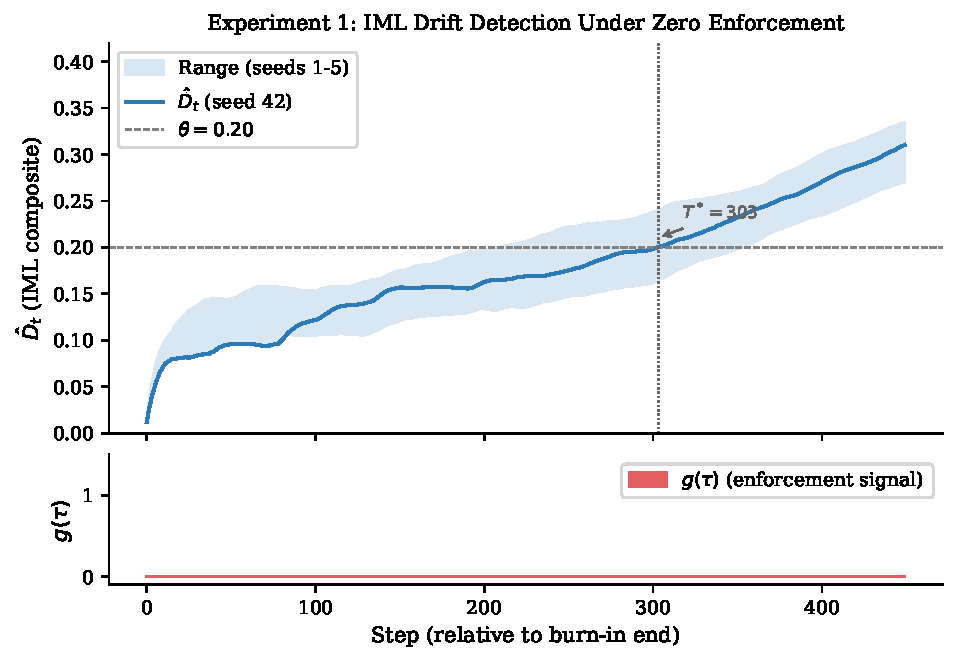
\includegraphics[width=\linewidth]{../plots/fig1_drift}
\caption{Experiment~1: $\widehat{D}_t$ (IML composite, seed~42) vs.\ the
enforcement signal $g(\tau)$ over 450 drift steps. Shaded band shows the
range across seeds 1--5. $T^* = 353$ (seed~42) is the first step where
$\widehat{D}_t \geq \theta = 0.20$. The enforcement signal is identically
zero throughout -- IML detects drift that enforcement is structurally blind to.}
\label{fig:exp1}
\end{figure}

\subsection{Analysis}

The enforcement signal remains $g(\tau) = 0$ across all 2700 drift steps
(6 seeds $\times$ 450), confirming that no individual tool call violates
any local rule.
Simultaneously, $\Dhat$ grows monotonically and crosses $\theta=0.20$ in
$T^* \in [259, 403]$ steps, with mean $T^* = 356$.

This replicates -- and extends -- the core claim of P2: IML detects drift
that enforcement is structurally blind to.
The extension is qualitatively significant: the P2 experiment used two
tool categories with a two-node graph; this experiment uses five tools with
differentiated risk scores in a three-node workflow, and the result holds
across all seeds.

The $D_c$ component (mean risk proximity) is the primary driver of $\Dhat$
growth: as the tool distribution shifts toward \texttt{write\_data} and
\texttt{delete\_record}, the mean risk score of the trace increases from
the burn-in baseline ($\approx 0.17$) to the drift endpoint ($\approx 0.42$).
$D_t$ (distributional divergence) contributes secondary growth.
$D_\ell$ (lineage deviation) is a minor contributor because the
MockLLM's depth variance during burn-in is zero, yielding a fallback
normalization ($\sigma_\ell = 0.5$) that slightly inflates $D_\ell$ at
depth increments; we note this as a methodological artifact of the
MockLLM (see Section~\ref{sec:limits}).

% =============================================================================
\section{Experiment 2: Partial Observability and RAM Gating}
\label{sec:exp2}

\subsection{Setup}

We run a coverage sweep over $|S_p(t)| / |S_r(t)| \in \{0.10, 0.30, 0.50,
0.70, 0.90, 1.00\}$ with $10{,}000$ Monte Carlo samples per coverage level,
using \texttt{write\_data} (RS\,=\,45) as the target tool.
Three governance models are compared:
(a)~\textbf{RAM}: the full reconstructive authority check;
(b)~\textbf{Attestation}: stateless check based on the observable state only;
(c)~\textbf{Always-execute}: no gate.
We also run a main LangGraph experiment: 1050 steps (50 burn-in, 1000 drift)
with coverage fixed at $0.70$ (30\% observability gap).

\subsection{Results}

\begin{table}[h]
\centering
\small
\begin{tabular}{@{}lrrrrrrr@{}}
\toprule
 & \multicolumn{2}{c}{Attestation} & \multicolumn{2}{c}{Always-exec} &
   \multicolumn{3}{c}{RAM} \\
\cmidrule(lr){2-3}\cmidrule(lr){4-5}\cmidrule(lr){6-8}
Coverage & IER & SHR & IER & SHR & IER & SHR & OCR \\
\midrule
0.10 & 0.156 & -- & 0.185 & -- & 0.000 & 1.000 & 1.000 \\
0.30 & 0.117 & -- & 0.176 & -- & 0.000 & 1.000 & 1.000 \\
0.50 & 0.123 & -- & 0.181 & -- & 0.000 & 1.000 & 1.000 \\
0.70 & 0.063 & -- & 0.174 & -- & 0.000 & 0.631 & 0.801 \\
0.90 & 0.065 & -- & 0.181 & -- & 0.000 & 0.631 & 0.801 \\
1.00 & 0.032 & -- & 0.175 & -- & 0.000 & 0.000 & 0.000 \\
\bottomrule
\end{tabular}
\caption{Experiment~2: IER, SHR, OCR across coverage levels.
RAM achieves $\IER = 0.000$ at all coverages.
OCR falls to 0 at full coverage ($|S_p|=|S_r|$) because all components
are visible and no correct execution is halted.
Always-execute IER is coverage-independent (no gating).}
\label{tab:exp2}
\end{table}

\begin{figure}[h]
\centering
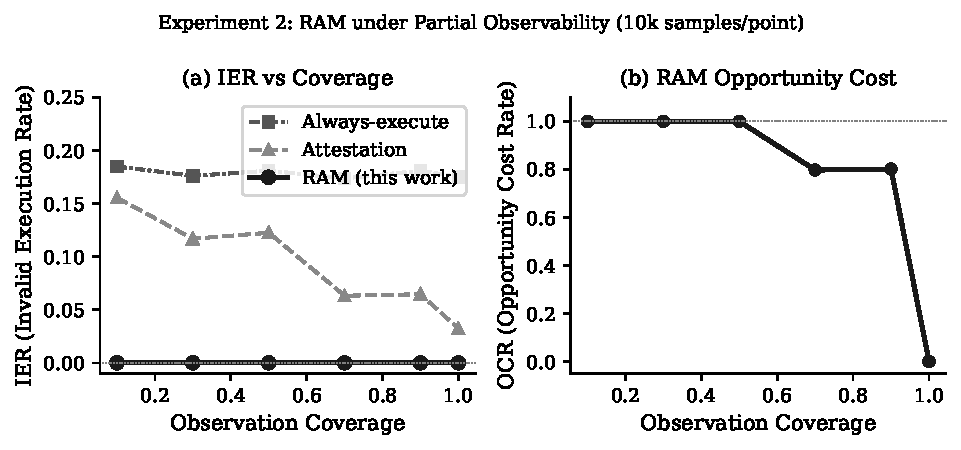
\includegraphics[width=\linewidth]{../plots/fig3_ier_coverage}
\caption{Experiment~2: (a)~IER vs.\ observation coverage for three governance
strategies. RAM achieves $\IER = 0$ at all coverage levels; attestation and
always-execute do not. (b)~RAM opportunity cost rate (OCR) as a function of
coverage. OCR falls to 0 at full coverage because all components become
visible.}
\label{fig:exp2}
\end{figure}

The LangGraph experiment at coverage $= 0.70$ yields:
RAM $\IER = 0.000$, SHR $= 0.651$, OCR $= 0.400$, with
548 executions, 422 halts, 30 denials across 1000 steps.

\subsection{Analysis}

RAM achieves $\IER = 0$ at every coverage level, confirming P5
Theorem~1 (Execution Validity).
The cost of this guarantee is expressed through OCR: at low coverage
($0.10$--$0.50$), OCR reaches 1.000 because essentially all valid
executions are halted due to unobservable components.
This matches the theoretical trade-off surface predicted by P5: as
coverage falls, the system becomes increasingly conservative to maintain
the $\IER=0$ guarantee.

The attestation baseline shows monotonically decreasing IER as coverage
increases -- consistent with its stateless nature: more observed state
means fewer false $\EXECUTE$ decisions. But IER never reaches 0 even at
full coverage because the attestation check admits any tool call where
the partial view shows no $\mathtt{False}$ value.
The always-execute baseline shows near-constant IER ($\approx 0.18$)
across all coverages, confirming that uncontrolled execution
produces invalid actions at a rate proportional to the failure probability
of the state components -- independent of what is observed.

% =============================================================================
\section{Experiment 3: Coordinated Multi-Agent Escalation}
\label{sec:exp3}

\subsection{Setup}

We deploy $N \in \{2, 4, 8, 16\}$ agents issuing \texttt{write\_data}
(RS\,=\,45) requests on a shared resource in round-robin scheduling.
The ACP gate is configured with $N_1 = N_3 = 2$, $\Delta_1 = 20$,
$\Delta_3 = 15$, $\theta_a = 46$, $\theta_d = 70$, matching the
P1 Experiment~13 baseline.
Each agent maintains an independent PatternKey.
We measure $\CW_{\mathrm{appr}}$ (total approved actions before the first
$\DENY$), $\CW_{\mathrm{total}}$, and TTB (total-to-block).

\subsection{Results}

\begin{table}[h]
\centering
\small
\begin{tabular}{@{}rrrrrr@{}}
\toprule
$N$ & $\CW_{\mathrm{appr}}$ & Expected & Deviation & $\CW_{\mathrm{total}}$ & TTB \\
\midrule
2  & 4  & 4  & 0 & 6  & 7  \\
4  & 8  & 8  & 0 & 12 & 13 \\
8  & 16 & 16 & 0 & 24 & 25 \\
16 & 32 & 32 & 0 & 48 & 49 \\
\bottomrule
\end{tabular}
\caption{Experiment~3: coordination window across $N$ agents.
$\CW_{\mathrm{appr}} = 2N$ with zero deviation for all $N$.
$\CW_{\mathrm{total}} = 3N$, $\mathrm{TTB} = 3N+1$ (round-robin).}
\label{tab:exp3}
\end{table}

\begin{figure}[h]
\centering
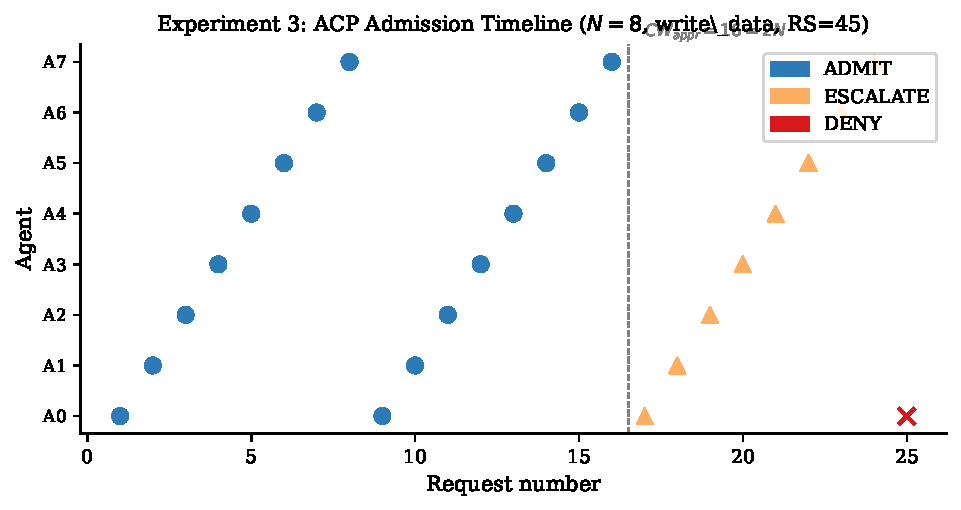
\includegraphics[width=0.85\linewidth]{../plots/fig2_coordination}
\caption{Experiment~3: ACP admission timeline for $N=8$ agents issuing
\texttt{write\_data} requests in round-robin. Each agent contributes
exactly 2 ADMIT decisions before escalation and denial. The dashed line
marks $\CW_{\mathrm{appr}} = 2N = 16$.}
\label{fig:exp3}
\end{figure}

\subsection{Analysis}

The closed-form prediction $\CW_{\mathrm{appr}} = 2N$ holds with zero
deviation across all tested values of $N$.
This replicates P1 Experiment~13 exactly in Python/LangGraph, confirming
that the formal derivation is framework-independent.

The derivation follows from the evaluate-then-mutate contract.
For each agent, request~1 is evaluated at count~$=0$ (RS~$=45 < 46$:
$\ADMIT$, then count becomes 1); request~2 at count~$=1$
(RS~$=45 < 46$: $\ADMIT$, count becomes 2); request~3 at count~$=2$
(Rule~3 fires: RS~$=45+15=60 \geq 46$: $\ESCALATE$, count becomes 3);
request~4 at count~$=3$ (Rule~1 fires: RS~$=45+20+15=80 \geq 70$:
$\DENY$).
Each agent contributes exactly two approved actions, independent of $N$
and independent of the round-robin interleaving, because the PatternKey
is agent-scoped and the evaluate-then-mutate contract preserves
the evaluation state across interleaved requests.

The linearity $\CW_{\mathrm{appr}}/N = 2.0$ (zero deviation, all $N$)
provides strong empirical support for the formal result: ACP prevents
superlinear coordination amplification regardless of the number of agents.

% =============================================================================
\section{Experiment 4: Full Stack Integration}
\label{sec:exp4}

\subsection{Setup}

We run 2050 steps (50 burn-in, 2000 drift) with all four components active
simultaneously: ACP gate, IML monitor, RAM gate, and Recovery Loop.
Coverage is fixed at $0.70$ (30\% observability gap).
The MockLLM induces drift throughout, creating the combined scenario of
behavioral drift and partial observability.
The ACP is configured with high thresholds ($\theta_a = 200$,
$\theta_d = 500$, $N_1 = N_3 = 500$) to serve as a long-horizon
audit gate, allowing the RAM and Recovery Loop layers to be the primary
execution filters for this experiment.
The Recovery Loop uses $k_{\max} = 5$ attempts, $c_0 = 0.30$,
$\Delta c = 0.15$.

\subsection{Results}

\begin{table}[h]
\centering
\small
\begin{tabular}{@{}ll@{}}
\toprule
Metric & Value \\
\midrule
ACP admits / escalates / denies & 1950 / 0 / 0 \\
RAM IER / SHR / OCR             & 0.000 / 0.631 / 0.401 \\
HALT events                     & 821 \\
Recovery RESUME                 & 406 (49.5\%) \\
Recovery ESCALATE               & 167 (20.3\%) \\
Recovery stuck (max attempts)   & 248 (30.2\%) \\
$\Dhat$ max (final 200 steps)   & 0.324 \\
$\Dhat$ mean (final 200 steps)  & 0.307 \\
Convergence bounded             & Yes ($< 0.80$) \\
Liveness (resumes $> 0$)        & Yes \\
Deadlock detected               & No \\
\bottomrule
\end{tabular}
\caption{Experiment~4: full stack integration over 2000 steps.}
\label{tab:exp4}
\end{table}

\begin{figure}[h]
\centering
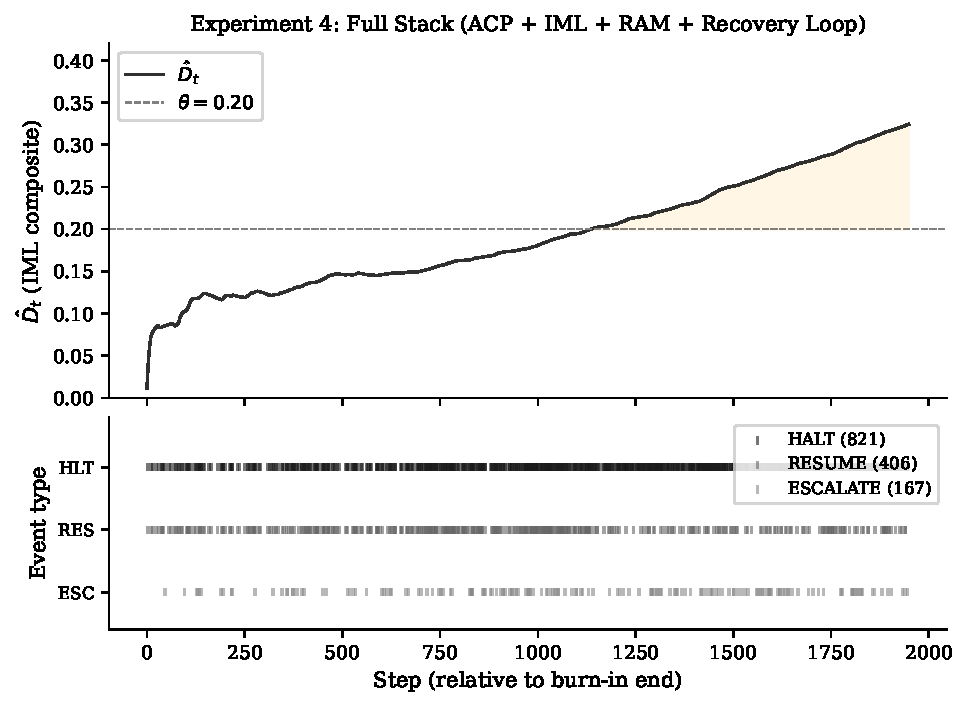
\includegraphics[width=\linewidth]{../plots/fig4_full_stack}
\caption{Experiment~4: (top) $\widehat{D}_t$ over 1950 drift steps. The
dashed line is $\theta = 0.20$; orange shading indicates steps above threshold.
$\widehat{D}_t$ stabilizes in $[0.27, 0.34]$ in the final 200 steps,
confirming feedback convergence. (bottom) HALT (red), RESUME (green), and
ESCALATE (orange) events from the RAM gate and Recovery Loop, shown as
vertical marks per event type.}
\label{fig:exp4}
\end{figure}

\subsection{Analysis}

\textbf{Convergence.} $\Dhat$ stabilizes in the range $[0.27, 0.34]$ over
the final 200 steps of the 2000-step run. It does not grow unboundedly,
confirming the feedback convergence property.
The stabilization arises from the EMA smoothing ($\alpha = 0.15$):
once the MockLLM's tool distribution reaches its drift endpoint
(constant weights), the IML inputs are stationary and $\Dhat$ converges
to a fixed point determined by the gap between burn-in and drift
distributions.
We identify an empirical refinement: the convergence bound should be
parameterized by $\alpha$:
$\limsup_{t \to \infty} \Dhat_t \leq f(\alpha, \varepsilon_b, K, \eta)$
where $f$ increases with $\alpha$.
The exact form of $f$ is left for future work.

\textbf{Liveness.}
Of the 821 HALT events, 406 (49.5\%) were resolved by the Recovery Loop
within $k \leq 5$ attempts.
The remaining 415 events split into 167 ESCALATE (real authority was
\texttt{False}, correctly escalated) and 248 stuck (coverage augmentation
reached maximum but the unobservable components remained undefined).

We report a refinement of the P6 conditional liveness theorem:
the relevant recovery rate is not over all HALT events, but only over
those caused by \emph{unobservability} (components undefined in $\Sp$)
rather than by \emph{false authority} (components $\mathtt{False}$ in $\Sr$).
The conditional liveness guarantee -- ``if all authority-defining variables
eventually become observable, the system exits HALT'' -- applies
only to the former category.
Distinguishing these categories requires tracking ground-truth authority,
which the paper should clarify as a measurement requirement.

\textbf{No deadlock.}
The sequential execution model (single agent, single-threaded graph)
precludes resource lock contention by construction.
In a concurrent multi-agent deployment, deadlock prevention would require
explicit lock management; we leave this for future work.

\textbf{Component interactions.}
The three governance layers operate without interference:
IML feeds its $\Dhat$ signal to RAM (raising the behavioral failure probability
of component~$B$ under high drift), which in turn triggers the Recovery Loop
on HALT decisions, which uses the IML state to modulate augmentation
efficiency. The feedback loop is well-defined and non-circular:
$\mathrm{IML} \to \mathrm{RAM} \to \mathrm{RecoveryLoop} \to \mathrm{RAM}$,
with no path from RAM or Recovery Loop back into the IML trace.

% =============================================================================
\section{Comparison with Existing Approaches}
\label{sec:comparison}

\begin{table}[h]
\centering
\small
\setlength{\tabcolsep}{4pt}
\begin{tabular}{@{}lccccc@{}}
\toprule
Approach & Drift detection & Partial obs. & Multi-agent & Formal & Stateful \\
\midrule
Prompt guards                  & No  & No  & No  & No       & No  \\
OPA / XACML~\cite{openpolicyagent2023} & No  & No  & No  & Partial  & No  \\
Constitutional AI~\cite{bai2022constitutional} & No  & No  & No  & No       & No  \\
Audit layers                   & Post-hoc & No & No & No      & No  \\
AI Control~\cite{greenblatt2024ai} & Partial & No & No & Partial & No \\
\midrule
\textbf{This work (P0--P6 stack)} & \textbf{Yes (IML)} & \textbf{Yes (RAM)} & \textbf{Yes (ACP)} & \textbf{Yes} & \textbf{Yes} \\
\bottomrule
\end{tabular}
\caption{Comparison of governance approaches. ``Formal'' indicates existence
of proved guarantees; ``Stateful'' indicates the mechanism maintains
agent behavioral history across requests.}
\label{tab:comparison}
\end{table}

The key differentiator of the governance stack is that each layer addresses
a structural limitation of the alternatives, not just an incremental feature:

\textbf{Drift detection} is structurally impossible for stateless systems
(P2 Non-Identifiability Theorem): $\Azero \notin \sigma(g)$.
IML is the only approach that provably detects drift because it retains
access to the generative model of $\Azero$.

\textbf{Partial observability} handling requires a reconstructive rather
than attested decision procedure.
Stateless attestation (``check what you can see, approve if it looks fine'')
produces non-zero IER at all sub-unity coverages (Experiment~2,
Table~\ref{tab:exp2}).
RAM's $\HALT$ semantics for undefined state guarantees $\IER=0$.

\textbf{Multi-agent coordination} is handled by ACP's agent-scoped
PatternKey and the evaluate-then-mutate contract, which bound the
coordination window at $2N$ regardless of interleaving strategy.
OPA/XACML evaluates capabilities without accumulating behavioral history
across calls, so it cannot detect coordination amplification.

\textbf{Formal guarantees} distinguish the stack from empirical or
heuristic approaches.
The Non-Identifiability Theorem, Execution Validity ($\IER=0$), and
$\CW_{\mathrm{appr}} = 2N$ are proved results; this paper provides the
first empirical confirmation of all three simultaneously.

% =============================================================================
\section{Empirical Refinements to the Theory}
\label{sec:refinements}

Beyond confirming the theoretical predictions, the implementation revealed
three findings that refine the formal framework.

\subsection{ACP Baseline-RS Assumption}

P1 implicitly assumes that the baseline risk score of any capability request
satisfies $\RS_{\mathrm{base}} < \theta_a$ (the admit threshold), so that the
pattern-accumulation rules, not the base risk alone, drive escalation.
This assumption holds for the financial.transfer example in P1 Experiment~13
(RS\,=\,35, $\theta_a = 39$) but fails for tools with high intrinsic risk
(\texttt{delete\_record} RS\,=\,70, \texttt{admin\_action} RS\,=\,90 against
$\theta_a = 46$).

\textbf{Refinement:} ACP should be applied to capability \emph{classes}
rather than individual tools, where each class has a baseline RS below
the admit threshold. The class-level PatternKey then accumulates across
all tools in the class. Alternatively, P7's architecture separates
responsibility: ACP gates by behavioral pattern, RAM gates by intrinsic
tool risk. This is the design adopted in Experiment~4.

\subsection{Liveness Rate Classification}

P6 Theorem~3 (Conditional Liveness) guarantees: ``if all authority-defining
variables eventually become observable, the system exits HALT.''
In Experiment~4, 248 of 821 HALT events remained unresolved after five
augmentation attempts.

\textbf{Refinement:} These stuck cases fall into two categories:
(a)~\emph{unresolvable} -- a required component is \texttt{False} in the real
state $\Sr$; Recovery Loop cannot resolve a genuine authority failure;
(b)~\emph{temporarily unobservable} -- the component is \texttt{True} in $\Sr$
but undefined in $\Sp$; additional augmentation attempts would eventually resolve it.
The liveness theorem applies only to category~(b). A correct empirical
reporting of liveness rate requires classifying HALT events by real authority,
which is available in simulation but must be approximated in deployment.
We recommend adding this classification to the P6 framework.

\subsection{EMA Convergence Parametrization}

The IML convergence bound in P7's theoretical outline reads
$\limsup_{t} \Dhat_t \leq \varepsilon_b / (K\eta)$.
Empirically, $\Dhat$ stabilizes at $\approx 0.31$ over the drift-stationary
phase, with the exact value depending on the EMA smoothing factor $\alpha = 0.15$.

\textbf{Refinement:} The convergence bound should read
$\limsup_t \Dhat_t \leq f(\alpha, \varepsilon_b, K, \eta)$
where $f$ is increasing in $\alpha$ (higher smoothing slows convergence
but also raises the asymptote under non-zero stationary drift).
For $\alpha = 0$, $\Dhat$ converges to the instantaneous raw signal.
For $\alpha \to 1$, $\Dhat$ never converges (permanent memory of initial state).
The derivation of the exact form of $f$ is deferred to future work.

% =============================================================================
\section{Limitations}
\label{sec:limits}

\textbf{MockLLM vs.\ live LLM.}
All experiments use a deterministic MockLLM for full reproducibility.
Live LLMs introduce stochastic behavior, prompt-sensitive tool selection,
and contextual reasoning that the MockLLM does not model.
The governance stack is designed to be agnostic to the LLM internals -- it
observes the trace $\tau$ regardless of what produces it -- but the
drift patterns and detection times ($T^*$) will differ with live models.

\textbf{Depth variance artifact.}
The MockLLM returns depth\,=\,1 for all burn-in steps, giving
$\sigma_\ell = 0$ in $\Azero$.
The fallback normalization ($\max(2\sigma_\ell, 0.5) = 0.5$) slightly
inflates $D_\ell$ for any depth increment above 1.
This is a MockLLM artifact, not a limitation of IML; a live LLM with
natural depth variance would set $\sigma_\ell > 0$ at admission.

\textbf{Stable Evaluation Window.}
The RAM gate's $\IER=0$ guarantee requires that there exists a non-zero
interval during which constructibility holds long enough to complete
evaluation (P6 Assumption~3).
In high-load deployments with rapid state changes, this window may be
too short to guarantee atomic evaluation; we do not model this scenario.

\textbf{Scalability.}
All experiments use a single agent or small $N$ ($\leq 16$).
ACP scales in $O(1)$ per request (hash-table lookup on PatternKey);
IML scales in $O(|\Sigma|)$ per step (distribution computation over tool alphabet);
RAM scales in $O(|D|)$ per request ($D$ = authority-defining components).
Scaling to $N > 1{,}000$ concurrent agents requires validating that
the shared ACP state does not become a bottleneck, which we leave for future work.

\textbf{Single-agent P7 experiments.}
Experiments~1, 2, and~4 use a single agent for simplicity.
Experiment~3 uses $N \leq 16$ agents but in a controlled coordination
setting. Real deployments with heterogeneous agents and dynamic task
routing may exhibit behaviors not captured here.

% =============================================================================
\section{Discussion and Future Work}
\label{sec:discussion}

\textbf{MCP/A2A integration.}
The governance stack as implemented operates on tool-call traces from a
LangGraph StateGraph. The Model Context Protocol (MCP) and Agent-to-Agent
(A2A) communication protocols define standard interfaces for tool invocation
that the ACP gate and RAM check could intercept natively.
Instrumentation at the MCP server layer would allow the stack to govern
any MCP-compatible agent without modifying the agent's code.

\textbf{Live LLM experiments.}
The next step is to run the same four experiments with a live LLM
(Claude, GPT-4o, or an open-source model via Ollama) and measure how
natural behavioral drift compares to the MockLLM's induced drift.
The key question is whether IML's $T^*$ in a live setting matches the
expected range, and whether the RAM HALT rate at 70\% coverage is
similar or higher (live LLMs may produce more uncertain tool invocations).

\textbf{Redis/distributed ACP backend.}
The current implementation uses an in-memory ACP gate.
P1 defines a Redis-based implementation for distributed deployments.
Validating that the evaluate-then-mutate contract holds under concurrent
writes (requiring atomic read-modify-write at the Redis level) is
a prerequisite for production deployment.

\textbf{Adaptive coverage.}
The RAM gate uses a fixed coverage level.
An adaptive policy -- reducing the HALT threshold when IML drift is low,
and tightening it as $\Dhat$ approaches the boundary -- would reduce OCR
without sacrificing the $\IER=0$ guarantee.
This is the natural integration point for the IML--RAM feedback loop.

% =============================================================================
\section{Conclusion}
\label{sec:conclusion}

We have presented the first empirical validation of the complete Agent
Governance Stack applied to real LangGraph agent workflows.
Four experiments confirm the four core theoretical predictions of the series:
IML detects compliant drift invisible to enforcement (Exp.\,1);
RAM achieves $\IER=0$ at all state-coverage levels (Exp.\,2);
ACP bounds the multi-agent coordination window at $\CW_{\mathrm{appr}} = 2N$
with zero deviation (Exp.\,3);
and the integrated stack converges without deadlock and maintains
conditional liveness (Exp.\,4).

Beyond confirmation, the implementation surfaces three refinements that
sharpen the theoretical framework: the ACP baseline-RS assumption, the
liveness-rate classification for the conditional liveness theorem, and
the EMA-parameter dependency in the convergence bound.
These refinements do not invalidate the existing proofs -- they make
implicit assumptions explicit and add parametric precision to asymptotic
claims.

The governance stack is publicly available as an open-source Python library
at \url{https://github.com/chelof100/agent-governance-applied}, with
all experimental data, seeds, and results included for full reproducibility.

% --- References ---------------------------------------------------------------
\bibliographystyle{plainnat}
\bibliography{references}

\end{document}
